\chapter{IPv4}
\label{chap:ipv4}

\section{Ejercicio 1.1}

\subsection{Muestra una captura del tráfico de paquetes DHCP intercambiados entre el nodo host[0] y los servidores
DHCP durante el proceso de obtención de su IP, obtenida en Wireshark (Nota: para que los tiempos mostrados
en Wireshark coincidan con los tiempos de simulación, activa Visualización → Formato de visualización de fecha
→ Segundos desde 1970-01-01). Explica lo que ocurre y para qué sirve cada paquete. Para facilitar la captura,
configura el startTime del cliente DHCP para que se inicie antes en host[0] que el resto de equipos}

\begin{figure}[!ht]
    \centering
    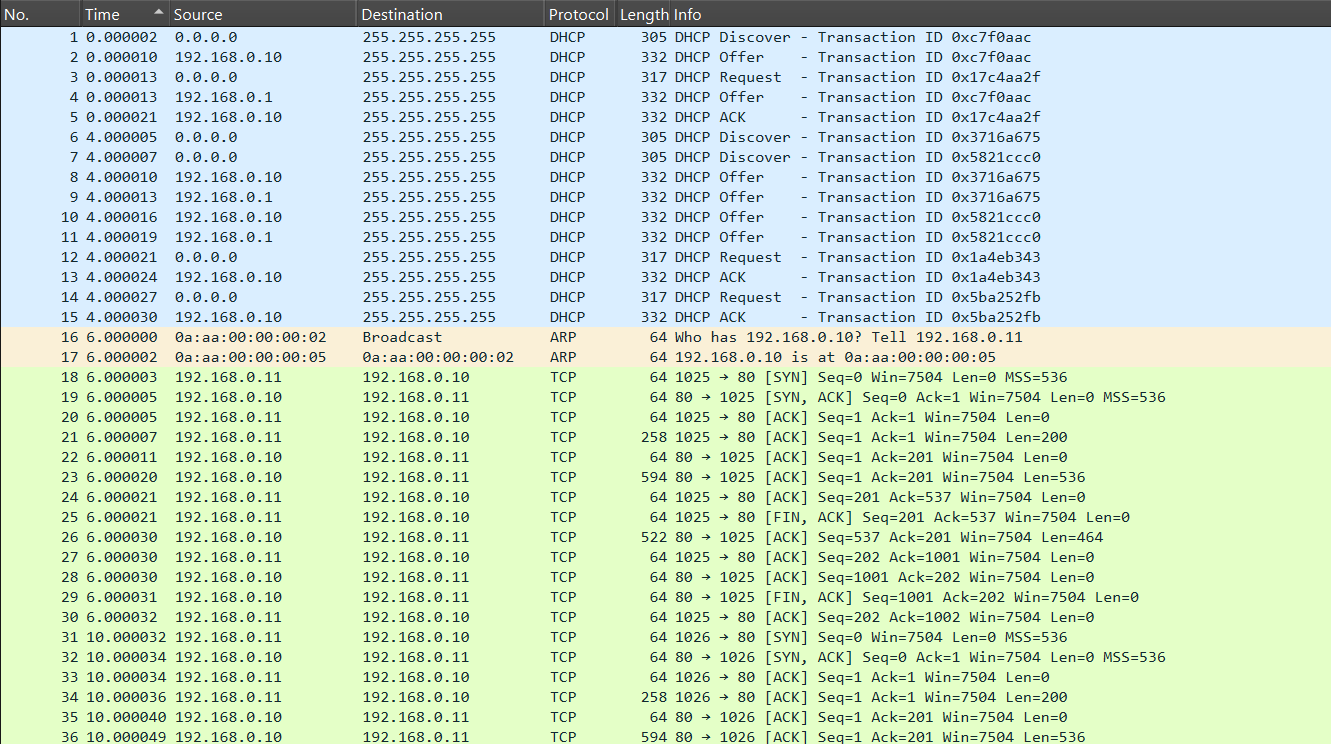
\includegraphics[width=135mm, scale=0.75]{imaxes/captura_ejer1_1.png}
    \caption{Tráfico DHCP entre host[0] y los servidores}
    \label{fig:captura_host0}
\end{figure}

Como podemos observar, el host[0] empieza haciendo un DHCP Discover para descubrir un servidor DHCP disponible. 
A continuación, el servidor local es el primero en responder la solicitud con un paquete DHCP Offer con una dirección IP disponible. El cliente (host[0]),
responde a su solicitud para confirmar la asignación ofrecida por el servidor local. El router también envía el paquete DHCP Offer, pero al enviarlo más tarde,
el cliente lo ignora. Finalmente, el servidor local contesta con un ACK (estos procesos se repiten para todos los cliente, host[1] y host[2]).

Posteriormente, el cliente host[0] intenta hacer la conexión con el servidor local, para lo cual manda primero un broadcast ARP, para asi saber 
cual es la MAC de la máquina, con la IP que establece en la cabecera ARP. Después, el servidor contesta al broadcast ARP que mandó el cliente identificandose su mac, ya que la cabecera ARP incluye su IP.

Finalmente, la conexión sigue adelante con los mensajes de la capa Trasporte correspondientes para la comunicación, restableciendose cada 4 segundos esa conexion (esto ocurre ya que establecemos un idleInterval de 4 segundos).

Tipos de paquetes:

\begin{enumerate}
    \item DHCP DISCOVER: Para ubicar servidores DHCP disponibles. El cliente (en este caso Host[0]) manda un paquete con IP destino la de broadcast global.
    \item DHCP OFFER: Respuesta del servidor a un paquete DHCPDISCOVER. El servidor enviará un paquete donde la ip de origen será la del propio servidor (192.168.0.10) aldestino 255.255.255.255
    \item DHCP REQUEST: Solicitud del cliente. Este paquete será la respuesta del cliente al anterior paquete. Esta comunicación sigue siendo broadcast ya que no tiene una dirección IP privada válida
\end{enumerate}


\section{Ejercicio 1.2}

\subsection{¿Cuál de los servidores proporciona la IP a host[0]? ¿Sabe el otro servidor que host[0] no cogió la IP ofrecida por él? ¿Cómo? (Muestra el contenido de los paquetes relevantes en Wireshark.)}


\section{Ejercicio 1.3}

\subsection{¿De qué tipo son los primeros paquetes que se intercambian a partir de t = 6 segundos? ¿Cuál es su objetivo?}

Los primero paquetes que se intercambian en a partir de 6s son paquetes ARP. Este paquete lo empieza mandando el cliente en modo broadcast para saber a que MAC le corresponde la IP que establece en la cabecera del paquete ARP. Posteriormente, el servidor local (el que tiene la IP de la cabecera ARP), responde enviando un paquete ARP de respuesta unicast al host con su dirección MAC. Sin este paso, no se podería establecer la conexión.

\section{Ejercicio 1.4}

\subsection{¿Cuáles son las direcciones origen y destino de estos paquetes (solicitud y respuesta)? ¿Tienen IP origen o destino? ¿Por qué?}

\section{Ejercicio 1.5}

\subsection{Configura el servidor DHCP en serverlocal con numReservedAddresses = 10 y el cliente DHCP en host[2]
para que arranque antes que los otros clientes DHCP. Esto hará que host[2] reciba la IP fija asignada a
serverlocal (192.168.0.10). ¿Ocurre algún error cuando el host[2] recibe la IP de serverlocal? Configura el
cliente TCP en host[0] para que se conecte a serverlocal y describe paso a paso qué ocurre durante el
establecimiento de conexión TCP a partir de t = 6 segundos debido a esta duplicidad.}

Configurando la red para que el host[2] reciba de primero la IP con un numReservedAddresses = 10, efectivamente recibe la IP estática del servidor local tal y como lo menciona en el enunciado y no ocurre ningún error aunque tengamos dos dispositivos con la misma IP. No obstante, aunque no ocurra ningún error, esto puede desencadenar problemas en la red ya que habería un confrito de IPs como por ejemplo problemas de rendimiento en la red (retrasos en el procesamiento de paquetería o aumento de tráfico ARP al no poder resolver la MAC del disposivo),  pérdida de conexión, inconsistencias en las tablas ARP, etc.

\begin{figure}[!ht]
    \centering
    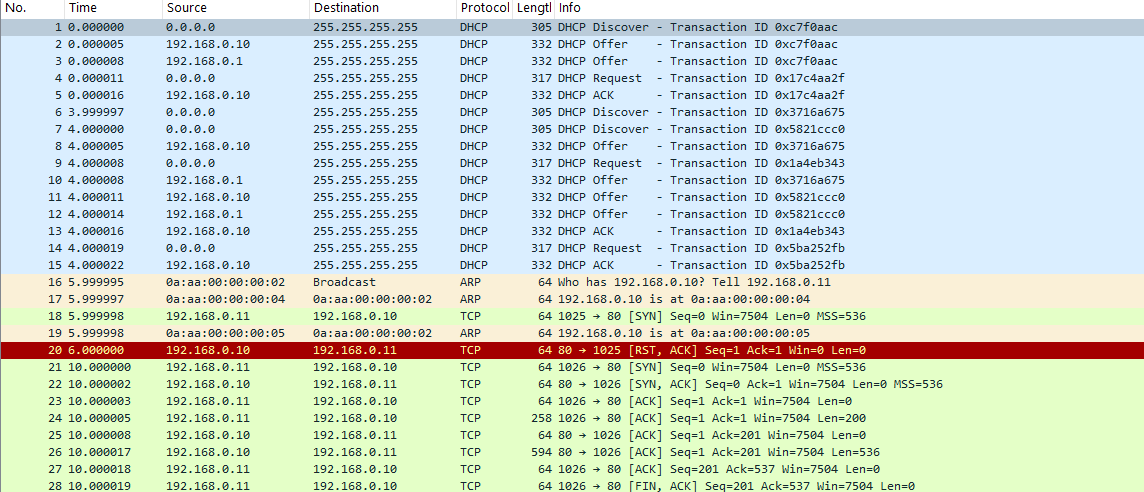
\includegraphics[width=135mm, scale=0.75]{imaxes/captura_ejer1_5.png}
    \caption{Tráfico DHCP entre host[0] y los servidores cuando host[2] recibe la ip servidor local}
    \label{fig:captura2_host0}
\end{figure}

Configurando el cliente TCP en el host[0], como se puede ver en la imagen \ref{fig:captura2_host0}, el host[0] manda un paquete ARP modo broadcast para averiguar la MAC del dispositivo con la ip 192.168.0.10. Le contesta primero el servidor local por lo que empieza la conexión en capa 4 pero poco después el host[2] contesta también al broadcast mandado por el host[0] ya que el tiene la misma IP asignada que el servidor local por lo que se interrumpe la conexión del host[0] con el servidor local mandando un RST,ACK. Pasados 4 segundos (ya que establecemos un idleInterval de 4 segundos), se vuelve establecer la conexión entre host[0] y el server local haciendose esta de manera exitosa ya que en la tabla ARP del host[0] se almacenó como dispositivo correspondiente a la IP 192.168.0.10, la MAC de servidor local ya que fue el primer dispositivo en responde al mandar paquetes ARP en modo broadcast 
